\documentclass[epsfig, a4paper,11pt,titlepage,openright]{book}
\usepackage[utf8]{inputenc}
\usepackage[italian]{babel}
\usepackage{amsmath}
\usepackage{amsfonts}
\usepackage{amssymb}
\usepackage{ragged2e}
\usepackage{graphicx}
\usepackage{epsfig}
\usepackage{plain}
\usepackage{setspace}
\usepackage[paperheight=29.7cm,right=2.5cm,left=3.5cm,top=2cm,bottom=2cm]{geometry} % per definizione layout
\usepackage{titlesec} % per formato custom dei titoli dei capitoli
\usepackage{float}

\usepackage[backend=biber,style=numeric,citestyle=authortitle, sorting=none]{biblatex}
\addbibresource{bibliografia.bib}

\linespread{1.25}

\begin{document}
	
	\frontmatter
	
	% nessuna numerazione
	
	\pagestyle{plain}

\thispagestyle{empty}

\begin{figure}[htbp]
	
\includegraphics[scale=1.3]{figure/logo.jpg}
	\label{fig}
\end{figure}
\vspace{2 cm}
 
\begin{center}
	\LARGE{Corso di Laurea in\\		
	\centering	
	\ Ingegneria Industriale
	}
	
	\vspace{1,5 cm} 
	\LARGE\textsc{PROVA FINALE\\} 
	\vspace{1 cm} 
	\LARGE\textit{Analisi di prestazioni di comfort di diverse strategie di controllo di sospensione semi-attiva\\}
	
	\vspace{1.5 cm} 
\end{center}


\begin{flushleft}
	\Large{Relatore}\\
	\Large{Prof. Giulio Panzani}\\
	\vspace{1.5 cm}
	\Large{Co-relatore}\\
	\Large{Prof. Giulia Giordano}\\
	\vspace{1.5 cm}
	\Large{Studente}\\
	\Large{Elia Bontempelli 201467}\\
\end{flushleft}


\begin{center}
	\vfill
	\Large{ANNO ACCADEMICO 2020/2021}
\end{center}

	
	\clearpage
	
	\chapter*{Ringraziamenti}
\label{cha:ring}
\textit{Vorrei dedicare questa tesi a tutte le persone che mi sono sempre state vicine e che mi hanno accompagnato in questi anni.}\\

\textit{In primis, un sentito grazie al mio relatore Panzani Giulio per la disponibilità mostrata, per avermi trasmesso la passione per questo ambito dell'Ingegneria e per essere stato fonte di conoscenza, sia come professore sia come guida per la realizzazione di questo lavoro.}\\

\textit{Ringrazio infinitamente i miei genitori che hanno sempre sostenuto me, mio fratello e mia sorella, appoggiandoci in ogni decisione e volendoci un bene dell'anima. Con i loro incredibili sforzi ci hanno permesso di portare avanti, con serenità, gli studi e tutti i nostri obiettivi. Soprattutto a loro voglio dedicare questo mio importante traguardo.}\\

\textit{Un ringraziamente speciale a Beatrice, perchè mi supporta in ogni momento e mi trasmette una forza incredibile. Grazie per esserci sempre.}\\

\textit{Grazie a Davide, Maria, Ivan, Gabriele, ai miei nonni e a tutti i parenti per il loro continuo sostegno e incoraggiamento.}\\

\textit{Infine, voglio ringraziare tutti gli amici e compagni di corso che sono stati presenti in questo viaggio e con i quali ho passato dei momenti indimenticabili ed indescrivibili.}\\

	
		
	
	\clearpage
	\pagestyle{plain} % nessuna intestazione e pie pagina con numero al centro
	
	\chapter*{Sommario} % senza numerazione
\label{sommario}

\addcontentsline{toc}{chapter}{Sommario} % da aggiungere comunque all'indice

Le sospensioni sono una delle parti fondamentali di un veicolo, costituiscono il collegamento principale tra la strada e il telaio e sono responsabili della sicurezza e del comfort del passeggero a bordo.\\
In questo lavoro sono state analizzate, tramite simulazioni su un modello quarter car, le prestazioni di comfort di diverse strategie di controllo per le sospensioni semi-attive di tipo magnetoreologico. La taratura dei parametri delle leggi di controllo è stata fatta tramite l'algoritmo di ottimizzazione bayesiana.\\
L'obiettivo iniziale era quello di osservare le prestazioni di due diverse leggi di controllo, lineare e quadratica, analizzarle in confronto a una configurazione passiva, e capire se l'algoritmo di ottimizzazione utilizzato fosse una tecnica efficiente per la taratura dei parametri. Nel corso del lavoro sono emersi però interessanti risultati e per questo si è voluto implementare un'ulteriore strategia di controllo, in modo da realizzare un'analisi più completa possibile.\\

Per la stesura della tesi si è fatto riferimento principalmente a \cite{controlMRdampers}.\\

Nella realizzazione di questa tesi sono stati utilizzati in parallelo i software MATLAB e Simulink. Quest'ultimo necessario per la realizzazione dello schema a blocchi del modello quarter car e per le simulazioni del sistema dinamico, mentre con l'ausilio di MATLAB sono stati elaborati i parametri necessari per il sistema dinamico, è stato implementato l'algoritmo di ottimizzazione e sono stati raccolti i dati delle simulazioni.\\




	
	\mainmatter

    % indice
    \tableofcontents


	\chapter{Introduzione}
\label{cha:intro}

Le sospensioni semi-attive sono costituite da ammortizzatori a smorzamento variabile e sono realizzate in modo tale che non sia possibile somministrare ulteriore energia meccanica al sistema, a differenza delle sospensione attive che sono costituite da attuatori che esercitano  una forza indipendente.\\
Le sospensioni semi-attive offrono affidabilità e prestazioni migliori rispetto alle sospensioni passive, mantenendo allo stesso tempo l'efficienza e l'ottima versatilità dei sistemi attivi, senza però aver bisogno di fonti di energia, rendendo possibile un risparmio dal punto di vista economico.\\

Il tipo di sospensione semi-attiva preso in esame in questa tesi è quello costituito da ammortizzatori che sfruttano gli effetti magnetoreologici di alcuni fluidi, come l'olio. La peculiarità di questi fluidi è che possono variare la propria viscosità in base all'azione di campi magnetici esterni, la cui intensità può essere facilmente regolata da un semplice circuito elettromagnetico. In questo modo è possibile modificare la forza di smorzamento esercitata dalla sospensione, senza cambiare la sua geometria. Controllare questo tipo di sospensione è un compito non banale, in quanto anche nella configurazione passiva, cioè quando l'ingresso di controllo è mantenuto costante, la sospensione magnetoreologica fornisce un comportamento non lineare.\\

\section{Modello quarter car}
L'analisi del comportamento dinamico di un veicolo può rivelarsi molto complessa, per questo si utilizzano dei modelli semplificati. Uno dei principali è il modello quarter car che descrive la dinamica verticale di un quarto dell'intero veicolo, concentrando l'analisi su una singola ruota e sul relativo sistema di sospensioni, trascurando le interazioni tra le varie parti del veicolo. Questo tipo di modello, rappresentato in \figurename \  \ref{fig:quarter-car}, è caratterizzato da una massa sospesa \textit{$m_s$}, corrispondente a un quarto della massa del telaio del veicolo e da una massa non sospesa \textit{$m_u$} che rappresenta la ruota. Queste due sono connesse dalla sospensione, modellata da una molla elastica di costante \textit{k} e dall'elemento \textit{$f_d$} che rappresenta lo smorzatore magnetoreologico. Inoltre, la molla elastica \textit{$k_t$}, posta tra massa non sospesa e profilo stradale, descrive la rigidezza della ruota.
\begin{figure}[hbt]
	\centering
	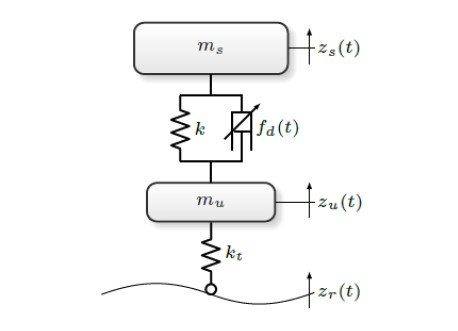
\includegraphics[scale=0.8]{figure/modello-quarter-car.jpg}
	\caption{Rappresentazione schematica del modello quarter car}
	\label{fig:quarter-car}
\end{figure}\\
Il modello matematico che descrive lo schema rappresentato in \figurename \ \ref{fig:quarter-car} può essere ottenuto considerando la legge di Newton per ognuna delle due masse, \textit{$m_s$} e \textit{$m_u$}, che si muovono lungo l'asse verticale. Le equazioni differenziali sono dunque le seguenti:
\begin{equation}
	\centering
	\begin{cases}
		m_s\ddot{z}_s = -k\tilde{z} - f_d(\dot{\tilde{z}})\\
		m_s\ddot{z}_u = -k_t(z_u - z_r) + k\tilde{z} + f_d(\dot{\tilde{z}}),\\
	\end{cases}
	\label{eqprinc}
\end{equation}\\
dove $\ddot{z}_s$, $\dot{z}_s$ e $z_s$ sono rispettivamente l'accelerazione, la velocità e lo spostamento della massa $m_s$ e $\ddot{z}_u$, $\dot{z}_u$ e $z_u$ sono l'accelerazione, la velocità e lo spostamento della massa $m_u$. Mentre $\tilde{z} := z_s - z_u$, $\dot{\tilde{z}}$ è la velocità di avanzamento e $z_r$ rappresenta il profilo stradale. Come detto pocanzi, \textit{$f_d$} è il termine che descrive la forza di smorzamento che introduce una forte non-linearità nel sistema.\\

Per lo svolgimento della tesi sono stati considerati valori numerici assimilabili a quelli di un SUV. Nella \tablename \ \ref{parametri} sono elencati i parametri del modello quarter car e della sospensione magnetoreologica.

\renewcommand\arraystretch{1.4} 
\begin{table}[hbt]
	\centering
	\begin{tabular}{|c||c|c|}
		\hline
		\textbf{Parametro} & \textbf{Simbolo} & \textbf{Valore} \\
		\hline	Massa della Ruota & \textit{$m_u$} & 70 \textit{Kg}\\
		\hline	Massa di $\frac{1}{4}$ di Veicolo & \textit{$m_s$} & 450 \textit{Kg}\\
		\hline	Rigidezza Sospensione & \textit{$k$} & 27000 \textit{$\frac{N}{M}$}\\
		\hline	Rigidezza Ruota & \textit{$k_t$} & 300000 \textit{$\frac{N}{M}$}\\
		\hline	Smorzamento minimo & \textit{$c_{min}$} & 800 \textit{$\frac{N s}{M}$}\\
		\hline	Pendenza di saturazione & \textit{$k_0$} & 38000 \textit{$\frac{N s}{M}$}\\
		\hline	Livello massimo di saturazione & \textit{$\tilde{f}_{max}$} & 3000 \textit{N}\\		
		\hline
	\end{tabular}
	\caption{Parametri modello quarter car e sospensione MR}
	\label{parametri}
\end{table}


\section{Implementazione modello in MATLAB \& Simulink}
Il passo successivo è stato quello di implementare in Simulink il modello quarter car del veicolo, secondo il sistema di equazioni \ref{eqprinc}. Con l'utilizzo di MATLAB sono stati definiti tutti i parametri utili, sono state lanciate tutte le simulazioni e sono stati raccolti tutti i risultati.\\
\begin{figure}[hbt]
	\centering
	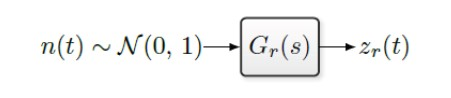
\includegraphics[scale=0.5]{figure/zr.jpg}
	\caption{Schema generazione profilo stradale}
	\label{fig:zr}
\end{figure}\\
La variazione del profilo stradale rappresenta l'input esterno del sistema ed è stato calcolato, come mostra la \figurename \ \ref{fig:zr}, filtrando un rumore gaussiano $n(t)$, attraverso la funzione di trasferimento $G_r(t)$ \eqref{Gr}. Questo tipo di approccio, utilizzato da \cite{controlMRdampers}, per definire il profilo stradale, è un'implementazione equivalente alla generazione di un profilo stradale secondo la normativa ISO-8608.
\begin{equation}
	\centering
	G_r(s) = \frac{s}{s^2 + 2\xi_r\omega_rs + \omega_r^2}
	\label{Gr}
\end{equation}
dove $\xi_r = 0.7$ e $\omega_r$ dipende dalla velocità del veicolo secondo la formula:
\begin{equation}
	\centering
	\omega_r = \frac{2\pi v}{l_c}
	.
	\label{omega_r}
\end{equation}
Il parametro $l_c$ è costante e rappresenta la massima risoluzione spaziale considerata, dove un valore piccolo del parametro corrisponde a considerare una strada quasi piatta con delle micro-asperità distribuite. La velocità considerata per tutte le simulazioni è pari a $v = 90\frac{km}{h}$.\\
In \figurename \ \ref{fig:profilostradale} è mostrato un esempio del profilo stradale ottenuto in MATLAB.
\begin{figure}[hbt]
	\centering
	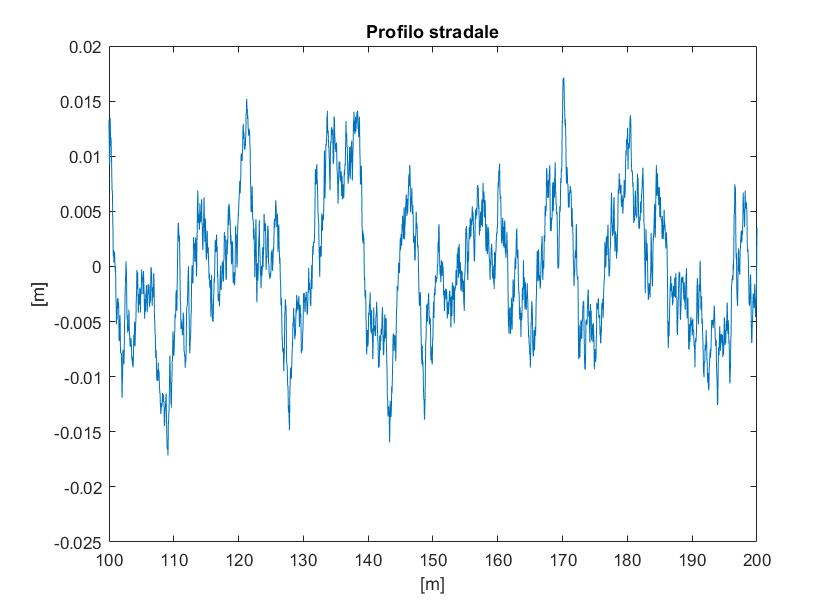
\includegraphics[scale=0.3]{figure/profilostradale.jpg}
	\caption{Esempio grafico profilo stradale}
	\label{fig:profilostradale}
\end{figure}\\
Il profilo stradale viene generato a seguito di un processo casuale, quindi i risultati possono variare da una simulazione all'altra. Per evitare una variabilità troppo alta, è stata considerato un tratto di strada sufficentemente lungo, di 2.5$km$.\\

Riepilogando, il sistema dinamico ha come ingresso la variazione del profilo stradale $z_r$, il vettore delle variabili di stato è definito come $x = [\dot{z_s}\ z_s\ \dot{\tilde{z}}\ \tilde{z}]^T $, mentre l'uscita corrisponde all'accelerazione verticale $\ddot{z_s}$ di $\frac{1}{4}$ del veicolo.\\
Il termine $f_d(\dot{\tilde{z}})$ che descrive la relazione di non-linearità tra forza dello smorzatore MR e velocità di avanzamento, presente in \eqref{eqprinc}, è definito dalla seguente equazione:
\begin{equation}
	\centering
	f_d = c_{min}*(\dot{z_s}-\dot{z_u}) + \tilde{f_d}(u_{MR},\dot{z_s}-\dot{z_u})
	.
	\label{fd}
\end{equation}
L'equazione \eqref{fd} è composta da un termine lineare, il quale rappresenta il minimo smorzamento, e dal termine $\tilde{f_d}$ che descrive la nonlinearità della sospensione ed è definito come:
\begin{equation}
	\centering
	\tilde{f_d}(u_{MR},\dot{z_s}-\dot{z_u}) = sat_{u_{MR}}(k_0(\dot{z_s} - \dot{z_u}))
	,
	\qquad\qquad u_{MR} \epsilon [0,\tilde{f}_{max}]
	\label{fdtilde}
\end{equation}
\'E importante notare come nell'equazione \eqref{fdtilde}, la variabile di controllo $u_{MR}$ della sospensione semi-attiva è definita in modo esplicito e corrisponde ai limiti della saturazione.\\	

Le prime simulazioni, fatte per familiarizzare meglio con il simulatore, sono state svolte con una configurazione passiva, cioè quando l'ingresso di controllo è mantenuto costante per tutta la durata della simulazione, e solo in un secondo momento è stata implementata la legge di controllo.

\section{Indice di performance \textit{J}}
\begin{figure}[htb]
	\centering
	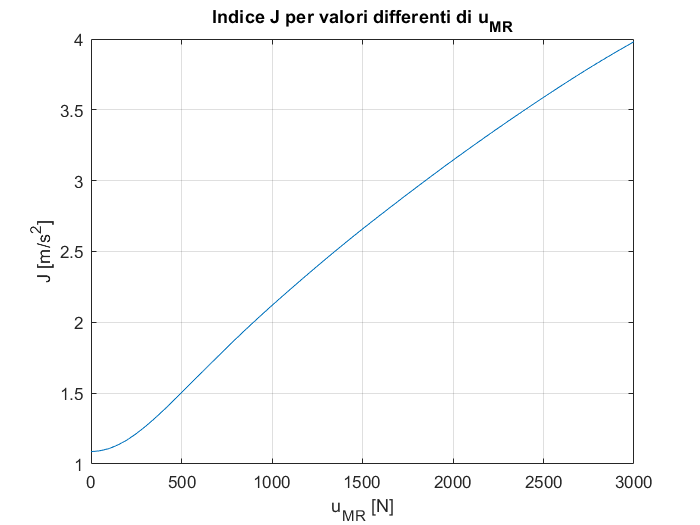
\includegraphics[scale=0.5]{figure/indice_performance.png}
	\caption{Indice di comfort per valori costanti differenti della variabile di controllo $u\textsubscript{MR} \epsilon [0,\tilde{f}_{max}]$}
	\label{fig:indiceperformance}
\end{figure}
Ci sono diversi modi per analizzare i dati di una simulazione e trarre delle conclusioni significative. Nel corso di questo lavoro è stata fatta particolare attenzione al valore dell'indice di performance, che corrisponde al valore dell'output del sistema $y = \ddot{z}_s$, come mostrato nell'equazione \eqref{indiceJ}.\\
Il confronto base per ogni strategia di controllo semi-attiva è la sospensione con una configurazione passiva e in questo caso è stato fatto in termini di comfort del passaggero, grazie all'indice \textit{J}.
\begin{equation}
	\centering
	J(\ddot{z}_s) = \left(\frac{1}{T}\int_{0}^{T}\lvert \ddot{z}_s(\tau) \rvert ^2 d\tau\right)^\frac{1}{2}
	\label{indiceJ}
\end{equation}
In \figurename \ \ref{fig:indiceperformance} è possibile visualizzare meglio l'andamento dell'indice \textit{J} in funzione di diversi valori della variabile di controllo $u_{MR}$. Si può notare come le prestazioni migliori, ${J\approx1.1\frac{m}{s^2}}$, siano ottenute con $u_{MR}\approx0$.


\section{Validazione del modello}
Per essere certi di aver fatto tutto correttamente, è stato necessario validare il modello implementato in Simulink con dei controesempi. In un primo momento sono state analizzate le simulazioni lineari, con $u_{MR}=0$, che risultano essere più semplici da verificare. Infatti, se $u_{MR} = 0$, il termine $\tilde{f}_d$ nell'equazione \eqref{fd} si annulla e quindi il modello non lineare si trasforma in uno lineare. Il blocco \textit{Space-State} di Simulink permette di implementare in modo semplice un sistema dinamico lineare: è sufficiente indicare le quattro matrici A, B, C e D che lo caratterizzano e l'input del sistema.  
\begin{equation}
	\centering
	\begin{cases}
		\dot{x} = Ax + Bz_r\\
		y = \ddot{z}_s = Cx + Dz_r\\
	\end{cases}
	\label{sistlineare}
\end{equation}

\begin{equation}
	\left[
	\begin{array}{c|c}
		A & B\\
		\hline
		C & D\\
	\end{array}
	\right] = \left[
	\begin{array}{c c c c|c}
		0 & 0 & 1 & 0 & 0\\
		0 & 0 & 0 & 1 & 0\\
		0 & -\frac{k}{m_s} & 0 & -\frac{c_{min}}{m_s} & 0\\
		\frac{k_t}{m_u} & -\frac{k}{m_s}-\frac{k_t + k}{m_u} & 0 & -\frac{c_{min}(m_s + m_u)}{m_um_s} & -\frac{k_t}{m_u}\\
		\hline
		0 & -\frac{k}{m_s} & 0 & 0 & 0\\
	\end{array}
	\right]
\end{equation}

A questo punto è stato confrontato l'output $\ddot{z}_s$ dei due sistemi, tramite il blocco \textit{Scope} che mostra l'andamento dei segnali in funzione del tempo della simulazione. L'accelerazione si è rivelata essere identica per entrambi i modelli, risultato che conferma la validità del simulatore realizzato.\\
Un' ulteriore analisi è stata fatta nel dominio della frequenza, dove è stata verificata l'uguaglianza delle funzioni di trasferimento dei due modelli. Per entrambi i sistemi è stata utilizzata la funzione \textit{tfestimate} di Matlab e come si evince dalla \figurename \ \ref{fig:Fdtconfronto}, i due grafici sono risultati essere perfettamente uguali.
\begin{figure}[hbt]
	\centering
	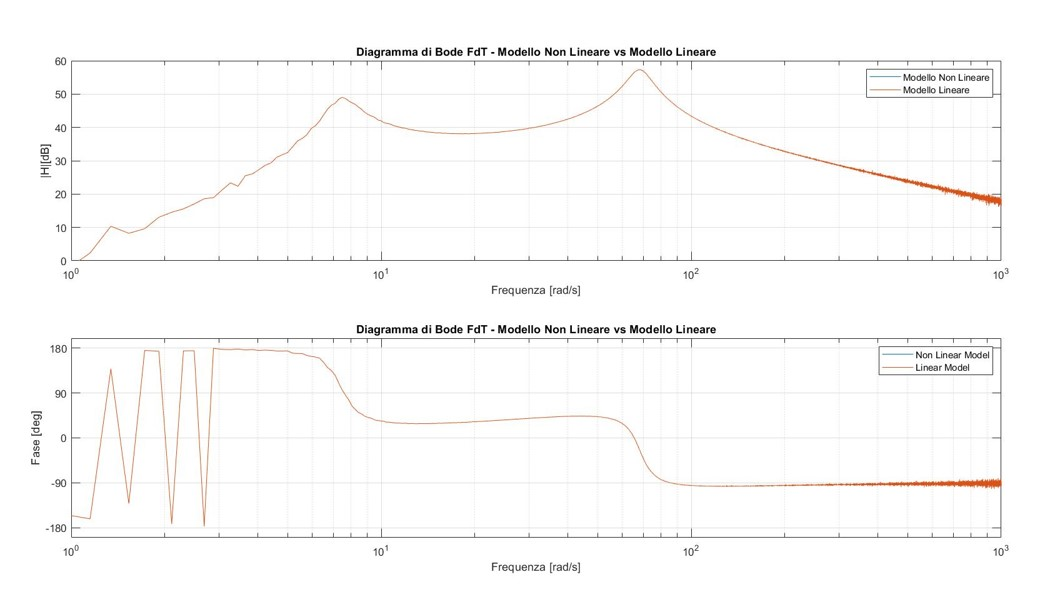
\includegraphics[scale=0.7]{figure/FdTconfronto.jpg}
	\caption{Confronto Funzione di Trasferimento modello lineare e non lineare}
	\label{fig:Fdtconfronto}
\end{figure}

Per quanto riguarda le simulazioni "non-lineari", con $u_{MR}\neq0$, è stato fatto un grafico della forza della sospensione in funzione della velocità di stroke $\dot{z}_s - \dot{z}_u$ e si è verificata l'uguaglianza con le mappe attese, vedi \cite{controlMRdampers}.
\begin{figure}[hbt]
	\centering
	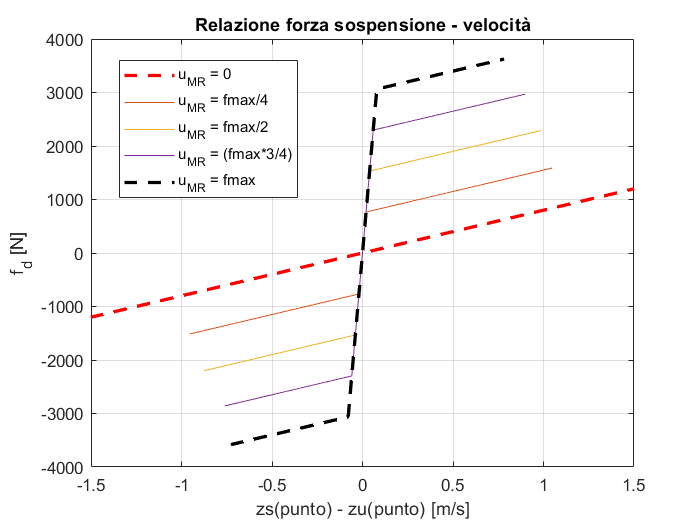
\includegraphics[scale=0.45]{figure/force-speed graph.png}
	\caption{Relazione tra forza e velocità della sospensione MR, con diveri valori di $u_{MR}$}
	\label{fig:graficofd}
\end{figure}

\section{Legge di controllo}
Una volta che il modello in Simulink è stato verificato ed è risultato corretto, il passo successivo e fondamentale per lo svolgimento della tesi è stato quello di implementare la legge di controllo.\\
In questo lavoro il controllore progettato per il sistema è un tipo di retroazione di stato standard, ottenuto a seguito di alcune manipolazioni, necessarie per poter essere applicato alla dinamica delle sospensioni MR, come mostrato in \cite{controlMRdampers}.\\
Nel corso di questa tesi sono state analizzate inizialmente le prestazioni di due diverse leggi di controllo, una di tipo lineare \eqref{leggelin} e una quadratica \eqref{leggequad}. A seguito però dei risultati ottenuti nel caso lineare e in quello quadratico, che saranno presentati successivamente, si è voluto implementare un'ulteriore legge di controllo, ottenuta sommando il termine lineare con quello quadratico \eqref{leggelinquad}. Le rispettive equazioni della variabile di controllo $u_{MR}$, che generano l'effettiva forza $\tilde{f}_d$ della sospensione, risultano essere:
\begin{equation}
	\centering
	u_{MR} = \frac{\tilde{f}_{max}}{2} + sgn(\dot{\tilde{z}})sat_{\frac{\tilde{f}_{max}}{2}}(\tilde{k}x),
	\label{leggelin}
\end{equation}
\begin{equation}
	\centering
	u_{MR} = \frac{\tilde{f}_{max}}{2} + sgn(\dot{\tilde{z}})sat_{\frac{\tilde{f}_{max}}{2}}(xP_xx^T),
	\label{leggequad}
\end{equation}
\begin{equation}
	\centering
	u_{MR} = \frac{\tilde{f}_{max}}{2} + sgn(\dot{\tilde{z}})sat_{\frac{\tilde{f}_{max}}{2}}(\tilde{k}x + xP_xx^T).
	\label{leggelinquad}
\end{equation}
I termini $\tilde{k}$ e $P_x$ sono rispettivamente un vettore e una matrice simmetrica, rappresentano un guadagno di stato retroazionato, lineare e non lineare, e il valore degli elementi che li compongono sono stati calcolati tramite un algoritmo di ottimizzazione.\begin{equation*}
	\tilde{k} = [k_1 \ k_2 \ k_3 \ k_4]^T \ \ \ \ \ \ \ \
	P_x = 
	\begin{bmatrix}
		p_{1,1} & p_{1,2} & p_{1,3} & p_{1,4} \\
		p_{2,1} & p_{2,2} & p_{2,3} & p_{2,4} \\
		p_{3,1} & p_{3,2} & p_{3,3} & p_{3,4} \\
		p_{4,1} & p_{4,2} & p_{4,3} & p_{4,4}
	\end{bmatrix}
\end{equation*}

















	\chapter{Taratura dei parametri delle leggi di controllo}
\label{cha:1}
Il fulcro centrale della tesi è stato l'implementazione in MATLAB dell'algoritmo di ottimizzazione e il successivo confronto dei diversi risultati ottenuti.\\
La taratura dei parametri è stata fatta tramite l'algoritmo di ottimizzazione Bayesiana, che in \nobreakdash MATLAB si traduce nell'utilizzo della funzione \cite{bayesopt}.

\section{Cenni teorici sull'ottimizzazione bayesiana}
L'ottimizzazione Bayesiana è un algoritmo molto versatile, progettato per ottimizzare modelli a scatola nera, ovvero sistemi dove l'espressione analitica della funzione obiettivo è sconosciuta, così come le sue derivate.\\
L'obiettivo della BO è la risoluzione del problema di ottimizzazione $\underset{\theta}{min} \ J(\theta)$, ovvero trovare per quali valori di $\theta$ la funzione $J(\theta)$ è minimizzata. Il termine $\theta$ può essere rappresentativo di uno o anche più parametri, il cui valore è sconosciuto, ma dove è possibile raccogliere un insieme di misure $J(\theta_1), J(\theta_2), J(\theta_3), \dots, J(\theta_N)$. Inizialmente l'algoritmo genera la funzione obiettivo in modo casuale, la quale viene aggiornata dopo ogni iterazione, a seguito del calcolo di nuovi valori di $J(\theta)$. Questo tipo di approccio statistico fornisce la distribuzione di probabilità di $J(\theta)$ per ogni parametro $\theta$ e questa probabilità è usata per definire una funzione di acquisizione $A(\theta)$. Infatti, la scelta del nuovo parametro da provare per il calcolo dei successivi campioni $J(\theta)$ non è casuale, bensì corrisponde al valore per cui $A(\theta)$ è massimizzata (\figurename \ \ref{fig:BO}). La funzione di acquisizione può essere di diversi tipi, la più comune e anche quella utilizzata in questo lavoro nella \cite{bayesopt} di MATLAB, è la cosiddetta \textit{Expected Improvement (EI)}.\\
\begin{figure}[htb]
	\centering
	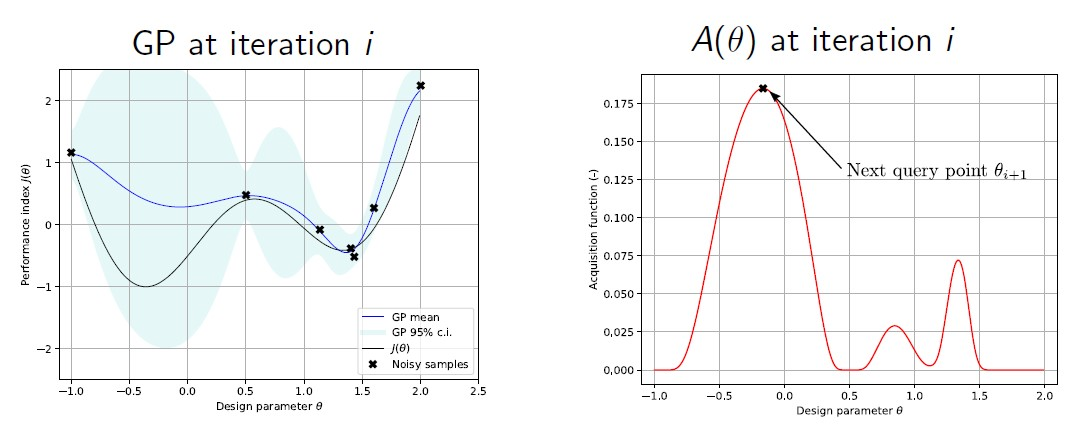
\includegraphics[scale=0.6]{figure/BO.jpg}
	\caption{Esempio di ottimizzazione bayesiana con modello surrogato e funzione di acquisizione}
	\label{fig:BO}
\end{figure}

Sebbene ci siano anche altri algoritmi che seguono principi simili, l'innovazione dell'ottimizzazione bayesiana sta proprio nel modo in cui il successivo punto di campionamento viene scelto e nel suo tentativo di convergere all'ottimo globale nel minor numero di iterazioni.\\
Grazie all'implementazione in MATLAB di questo tipo di ottimizzazione è stato possibile realizzare la taratura dei parametri per le due strategie di controllo, per le quali la cifra di costo che si vuole minimizzare è rappresentata dal valore efficacie dell'accelerazione verticale del veicolo. 

\section{Implementazione di \textit{bayesopt}}
La funzione di MATLAB \textit{bayesopt} richiede come input la funzione obiettivo che si vuole minimizzare e i parametri da ottimizzare. La cifra di costo richiesta come input corrisponde al calcolo dell'indice di performance $J$ per ogni simulazione. Nell'inizializzare le variabili da ottimizzare, che sono gli elementi del vettore $\tilde{k}$ e della matrice $P_x$, è necessario specificare il range di valori da esplorare per i diversi parametri, che a priori non è possibile conoscere, ma si può trovare a seguito di alcune simulazioni.\\
Considerando la legge lineare, l'argomento della saturazione in valore assoluto, nell'equazione \eqref{leggelin}, non può superare $\frac{\tilde{f}_{max}}{2}$, altrimenti risulterebbe un calcolo inutile. Sono state quindi fatte diverse simulazioni, con una configurazione passiva della sospensione, variando il valore di $u_{MR}$, in modo da calcolare il quantile al 95\% per ogni variabile di stato e poter poi trovare il range possibile per ogni parametro:
\begin{equation}
	\centering
	sat_{\frac{\tilde{f}_{max}}{2}}(\tilde{k}x) \  \Longrightarrow \  k_{i-max}*x_{i-max} = \frac{f_{max}}{2} \  \Longrightarrow \  k_{i-max} = \frac{f_{max}}{2}*\frac{1}{x_{i-max}}.
	\label{rangeparametri}
\end{equation}
In modo analogo sono stati i svolti i calcoli per trovare il range per i parametri della matrice $P_x$ della legge di controllo quadratica.\\

In MATLAB il codice necessario per implementare l'algoritmo di ottimizzazione risulta essere il seguente:
\begin{figure}[htb]
	\centering
	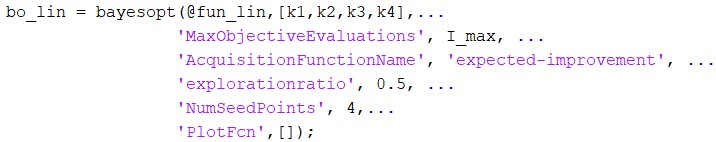
\includegraphics[scale=0.7]{figure/BOlin.jpg}
	\caption{Implementazione in MATLAB della funzione \textit{bayesopt}}
	\label{fig:bayesopt}
\end{figure}

\section{Analisi dei risultati}
Le simulazioni sono state fatte tutte con le impostazioni della \cite{bayesopt} mostrate in \figurename \ \ref{fig:bayesopt}. \textit{AquisitionFunctionName} indica il tipo di funzione di acquisizione utilizzata nell'algoritmo di ottimizzazione, l'\textit{explorationratio} fa riferimento alla propensione dell'algoritmo ad esplorare nuovi punti da campionare, più basso è, più si evita di "sprecare" iterazioni in punti non importanti, ma si rischia di rimanere bloccati in minimi locali. Infine, \nobreakdash\textit{NumSeedPoints} esplicita il numero di volte per cui si calcola la funzione di costo con parametri presi in modo casuale, nel range possibile indicato.\\
Sul grafico in \figurename \ \ref{fig:plotJ} è mostrato l'andamento della minimizzazione della funzione obiettivo $J$ in relazione al numero delle iterazioni.
\begin{figure}[htb]
	\centering
	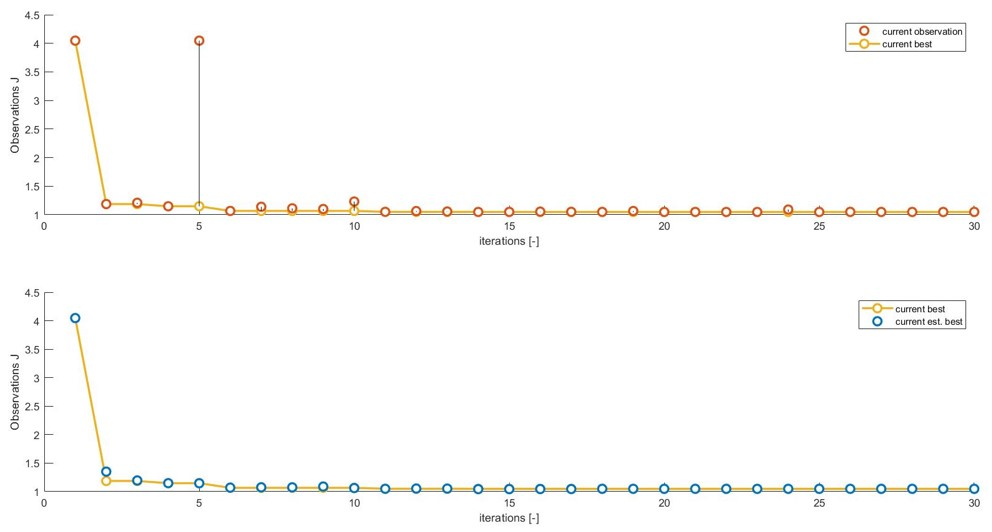
\includegraphics[scale=0.7]{figure/plotJ.jpg}
	\caption{Implementazione in MATLAB della funzione \textit{bayesopt}}
	\label{fig:plotJ}
\end{figure}\\
Per un'ottimizzazione più completa possibile, le simulazioni sono state eseguite con un numero di iterazioni sufficientemente elevato e per più volte tramite ciclo \textit{for}, in modo da osservare anche la variabilità dei risultati con un diverso ingresso $z_r$.\\

\subsection{Legge di controllo lineare}
\label{lin}
In \tablename \ \ref{risultatileggelin} è mostrato il resoconto di 10 diversi processi di ottimizzazione, per ognuno dei quali è stato generato un diverso input $z_r$. La tabella sottolinea come, in ogni simulazione, l'implementazione della legge di controllo lineare per la sospensione semi-attiva, faccia sì che l'indice di performance sia minore rispetto ad una configurazione passiva della sospensione. Questa è una prima dimostrazione di come una legge di controllo lineare vada a migliorare le prestazioni di comfort, rispetto ad una configurazione passiva della sospensione.\\
\'E possibile inoltre osservare, come i parametri $k_1, k_3$ e $k_4$, al variare delle simulazioni, abbiano rispettivamente dei valori molto simili, mentre il  parametro $k_2$ assuma  sempre dei valori molto differenti nelle diverse ottimizzazioni. Il fatto che $k_2$ vari molto indica che questo parametro, associato alla variabile di stato $z_s$ non è così fondamentale per la legge di controllo. Questa osservazione conferma ciò che potrebbe essere intuibile già "ad occhio nudo", ovvero che la posizione della macchina non ha nessuna influenza sul sistema e sulle sospensioni.\\
Questo risultato si è rivelato molto importante per il prosieguo del lavoro, infatti per le successive simulazioni, nella taratura dei parametri tramite ottimizzatore, è stato omesso il parametro $k_2$, semplificando quindi il problema e risparmiando tempo.\\
\renewcommand\arraystretch{1.4} 
\begin{table}[hbt]
	\centering
	\begin{tabular}{|c||c|c|c|c||c|c|}
		\hline
		$\# iterazioni$ & \textbf{$k_1$} & \textbf{$k_2$} & \textbf{$k_3$} & \textbf{$k_4$} & \textbf{$J_{ottim} \ [\frac{m}{s^2}]$} & \textbf{$J_{u_{MR} = 0} \ [\frac{m}{s^2}]$}\\
		\hline
		\hline 100 & 4994.7 & 1256.1 & -48964.9 & -57686.1 & 1.0410 & 1.0854\\
		\hline 100 & 4891.1 & 916 & -42489 & -52825 & 1.0600 & 1.1372\\
		\hline 100 & 4882.6 & -1068.2 & -45049.1 & -57644.7 & 1.0519 & 1.1044\\
		\hline 100 & 4832.6 & -1626.5 & -37832.2 & -52204.1 & 1.1003 & 1.1770\\
		\hline 100 & 5112.3 & -184.7 & -46131.6 & -56255.9 & 1.0662 & 1.1053\\
		\hline 100 & 4836.7 & 1862.5 & -39944.8 & -51648.3 & 1.0578 & 1.1528\\
		\hline 100 & 4778.6 & 1070.9 & -48280.1 & -55971.2 & 1.0671 & 1.1114\\
		\hline 100 & 4965.8 & 416.8 & -66707.4 & -58684.9 & 1.0560 & 1.0860\\
		\hline 100 & 4863.3 & -1386.5 & -43122.3 & -56622.4 & 1.0697 & 1.1130\\
		\hline 100 & 5027.5 & -1568.5 & -44443 & -55609.9 & 1.0613 & 1.1144\\		
		\hline
	\end{tabular}
	\caption{Taratura dei parametri per 10 simulazioni, eseguite con un diverso input $z_r$}
	\label{risultatileggelin}
\end{table}\\
L'analisi dei risultati più significativa e immediata risulta essere quella fatta nel dominio della frequenza, tracciando il grafico della funzione di trasferimento del modello implemetato con la legge di controllo e il modello con la configurazione passiva della sospensione. In questo modo è possibile apprezzare meglio la differenza tra i modelli, in termini di prestazioni di comfort (\figurename \ \ref{fig:confronto}).
\begin{figure}[htb]
	\centering
	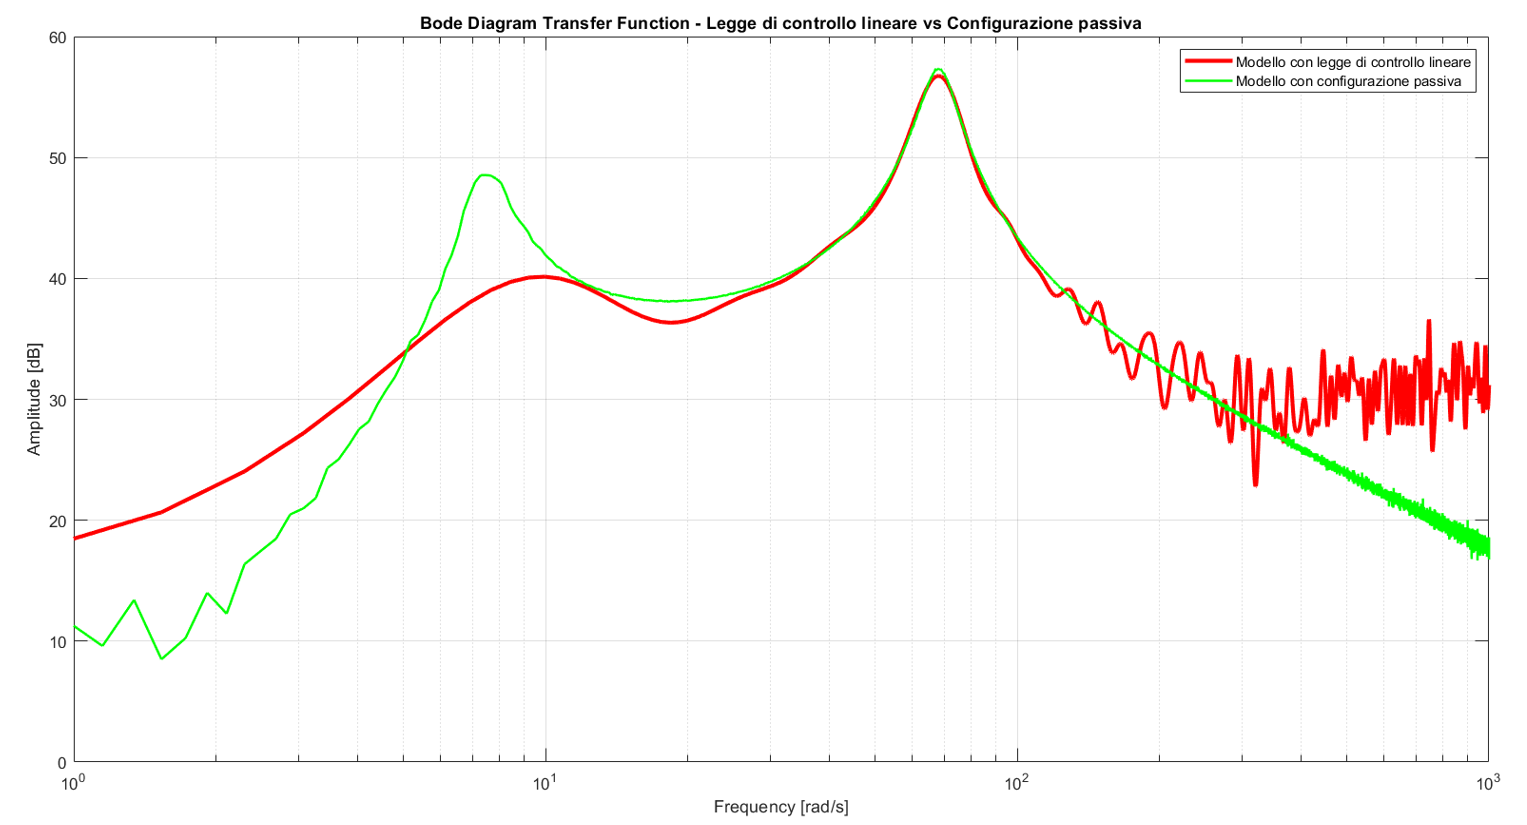
\includegraphics[scale=0.4]{figure/confrontoPas-Lin.png}
	\caption{Diagramma di Bode del modulo della FdT : modello con legge lineare e configurazione passiva}
	\label{fig:confronto}
\end{figure}\\
Dalla \figurename \ \ref{fig:confronto} la differenza tra i vari modelli è rimarcata soprattutto in corrispondenza del primo picco, dove per il modello implementato con la legge di controllo lineare, è decisiamente più smussato.\\
Ad alte frequenze risulta più difficile per la funzione \textit{tfestimate} stimare in modo preciso il modulo della funzione di trasferimento, in quanto ci si sta avvicinando alla frequenza di campionamento utilizzata e per questo sono presenti molte oscillazioni nel grafico.


\subsection{Legge di controllo quadratica}
\label{quad}
In modo analogo a quanto fatto per la legge di controllo lineare, è stata implementata la legge di controllo quadratica \eqref{leggequad}, con ottimizzazione dei parametri della matrice $P_x$. Essendo la matrice simmetrica 4x4 i parametri da ottimizzare sono 10 in tutto, ma avendo analizzato i risultati ottenuti per la legge lineare, si possono porre a zero tutti i termini che includono la variabile di stato $z_s$ e quindi ne consegue che gli elementi da ottimizzare sono: $p_{1,1}$, $p_{1,3}$, $p_{1,4}$, $p_{3,3}$, $p_{3,4}$, $p_{4,4}$.\\
In un primo momento i risultati ottenuti non sono stati così soddisfacenti, infatti, per ogni simulazione, il valore dell'indice di performance per il modello implementato con la legge di controllo quadratica risultava essere sempre maggiore rispetto al modello con configurazione passiva, circa $2.4\frac{m}{s^2}$.\\
A questo punto è stato fondamentale fare un'analisi di sensitività della cifra di costo in funzione delle dimensioni della "scatola", in cui l'ottimizzatore va a ricercare i parametri della legge di controllo. Sono state fatte ulteriori simulazioni aumentando, anche di diversi ordini di grandezza, il range di valori entro il quale l'algoritmo di ottimizzazione prende i parametri. Si è osservato che per tre ordini di grandezza in più rispetto ai valori limite, trovati tramite la formula \eqref{parametri}, il valore della cifra di costo migliora sensibilmente ($1.3\frac{m}{s^2}$), senza però riuscire ad ottenere un valore simile a quello ottenuto con una configurazione passiva.\\

\section{Osservazioni finali}
Tramite il modello controllato attraverso la legge quadratica non si sono raggiunti degli ottimi risultati, per quanto riguarda l'indice di performance, eppure il modulo della funzione di trasferimento ci ha fornito delle importanti informazioni sulle prestazioni di questa strategia di controllo. 
In \figurename \ \ref{fig:confrontolinquad} è possibile osservare la differenza, nel dominio della frequenza, tra il modello con una legge di controllo lineare e quello con legge di controllo quadratica. Se si considera tutto il campo di validità, una strategia di controllo lineare fornisce delle migliori prestazioni, così come indica l'indice $J$. Tuttavia, la legge di controllo quadratica fornisce migliori performance a frequenza basse e quindi presenta comunque una buona soluzione per alcuni casi particolari.\\
\begin{figure}[htb]
	\centering
	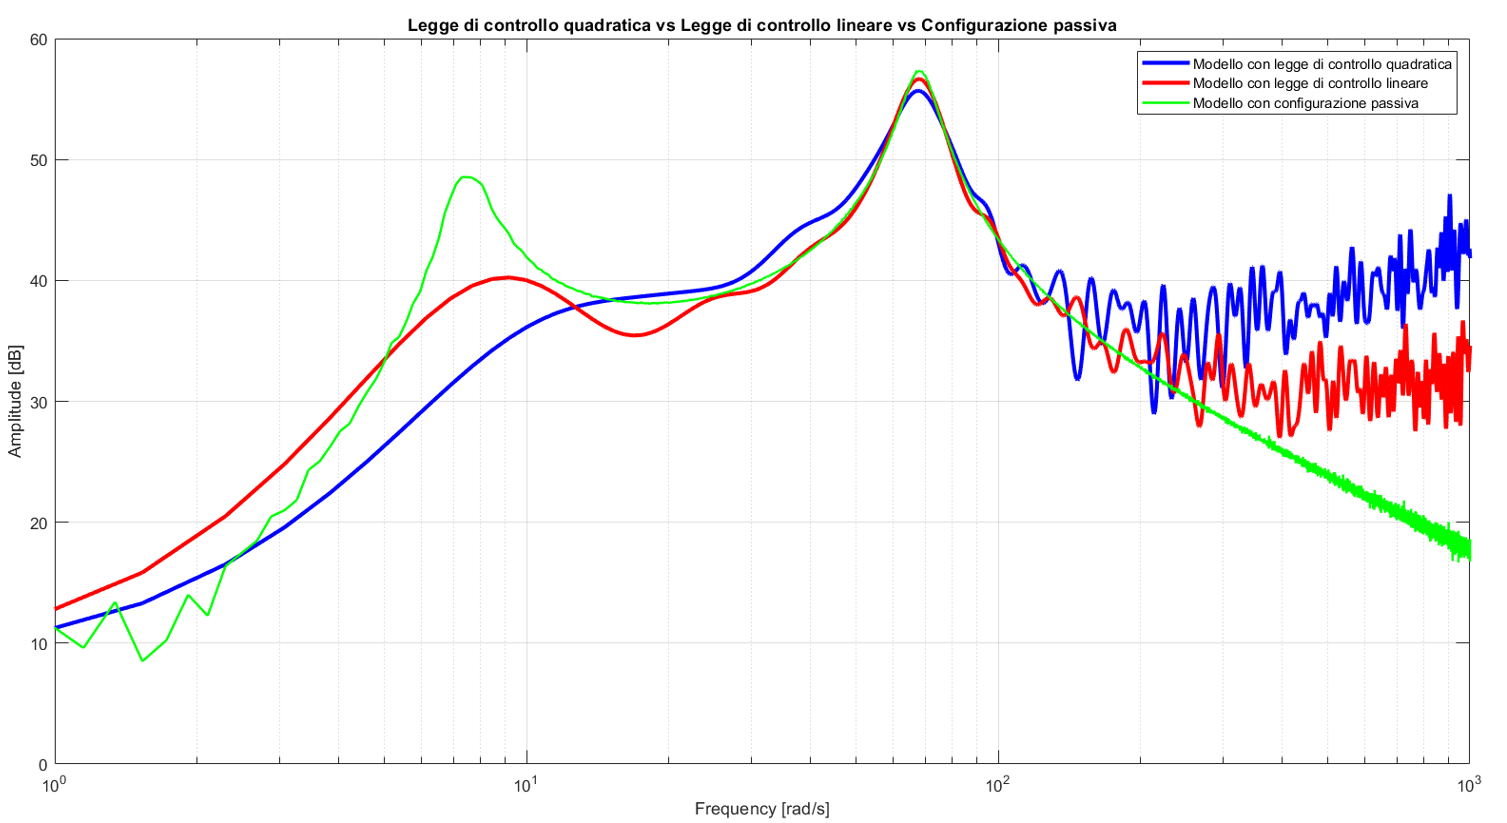
\includegraphics[scale=0.4]{figure/confrontoPas-Lin-Quad.png}
	\caption{Diagramma di Bode del modulo della FdT : modello con legge lineare, legge quadratica e configurazione passiva}
	\label{fig:confrontolinquad}
\end{figure}\\

\newpage
Considerando i risultati ottenuti con le due diverse strategie di controllo presentate pocanzi, si è voluto provare ad adottare una soluzione che combinasse la legge di controllo lineare e quella quadratica. L'obiettivo era quello di ottenere dei risultati che ci fornissero le migliori performance possibili a basse frequenze, come la legge quadratica, ma anche a medio-alte frequenze, secondo l'andamento della legge lineare. In Simulink è stato quindi implementato il modello rappresentativo dell'equazione \eqref{leggelinquad}.\\
Il valore dell'indice di performance ottenuto per questo modello è risultato molto simile a quello della legge lineare, però, come si puù osservare dal grafico in \figurename \ \ref{fig:confrontofinale}, in generale non si vedono miglioramenti importanti nel combinare le due leggi insieme.

\begin{figure}[htb]
	\centering
	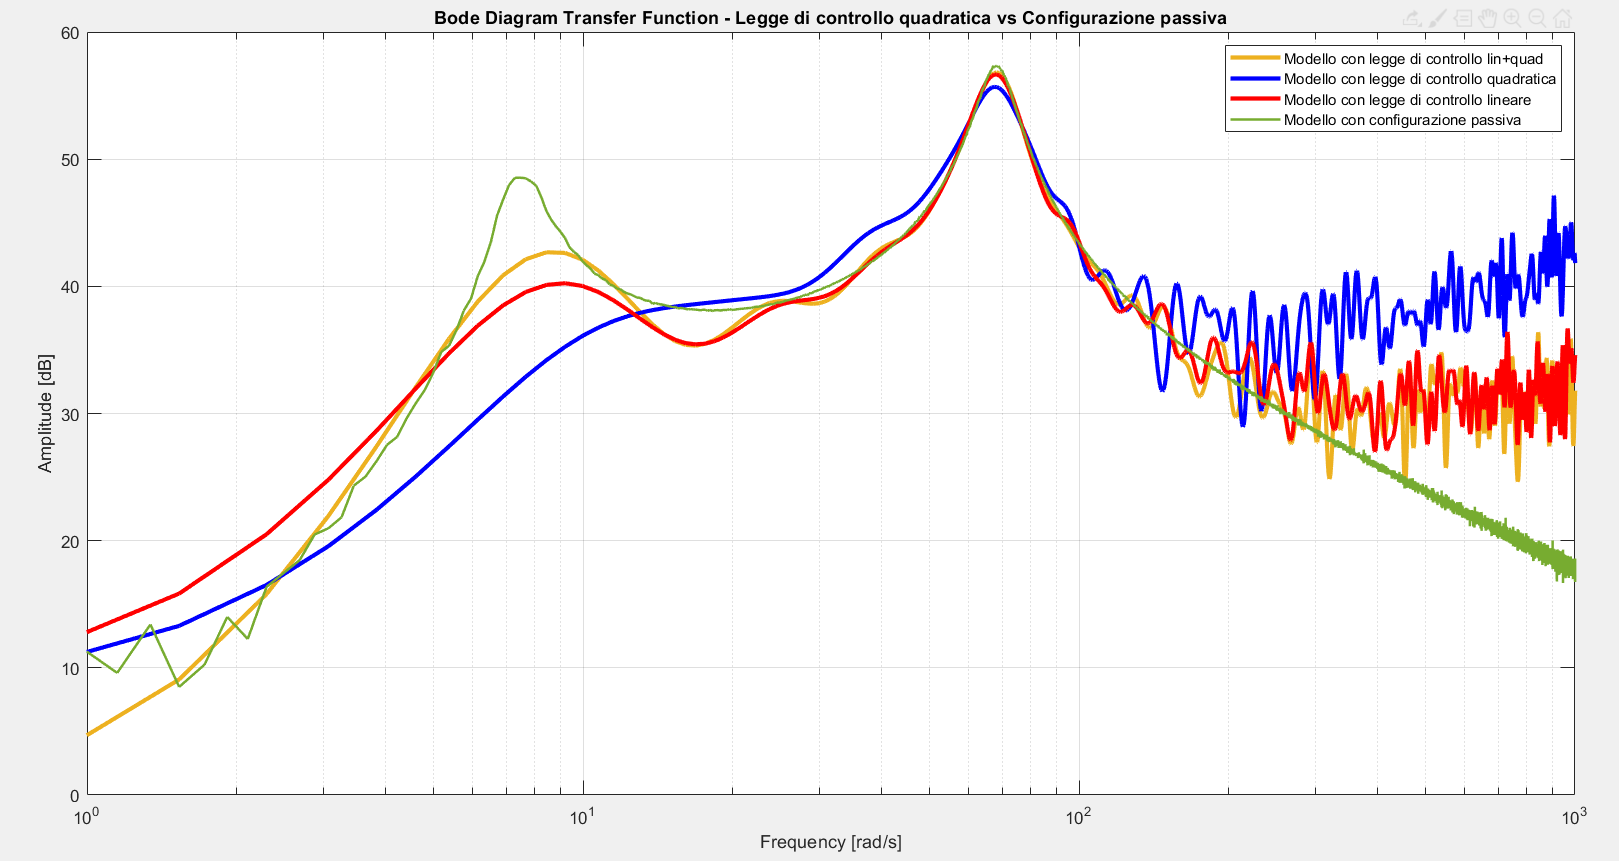
\includegraphics[scale=0.26]{figure/confrontofinale.png}
	\caption{Diagramma di Bode del modulo della FdT : confronto fra tutte le strategie di controllo implementate}
	\label{fig:confrontofinale}
\end{figure}




	\chapter{Conclusioni}
\label{cha:conclusioni}
Lo scopo di questa tesi è stato quello di approfondire l'implementazione in Simulink di un sistema dinamico e successivamente quello di ottimizzare, tramite l'algoritmo di ottimizzazione bayesiana, i parametri delle strategie di controllo.\\

In questo elaborato si è cercato di mettere in luce le differenze tra diverse strategie di controllo, analizzando soprattutto indice di performance e funzione di trasferimento, in modo da capire quale possa garantire delle prestazioni migliori in termini di comfort del passeggero e fornire quindi la soluzione migliore per il controllo di sospensioni semi-attive di tipo magnetoreologico.\\
La taratura dei parametri è stata fatta tramite l'utilizzo dell'algoritmo di ottimizzazione bayesiana, che ha fornito dei buoni risultati, ciò non esclude però che possano esserci delle tecniche migliori dell'ottimizzatore per trovare i valori corretti dei parametri delle leggi di controllo.\\

Lo svolgimento di questa tesi, mi ha dato l'opportunità di approfondire maggiormente, a livello pratico, temi legati al controllo di sistemi dinamici e la relativa implementazione, tramite software estremamente utilizzati in ambito ingegneristico.
	%\input{capitolo4}
     
    \backmatter
    
    
    
    

    \nocite{book1}
    \nocite{BO} 
    \addcontentsline{toc}{chapter}{Bibliografia e sitografia}
    \printbibliography[title = Bibliografia e sitografia]
    

\end{document}
